\documentclass[a4paper,11pt,singlespacing]{article}

\usepackage{setspace}
\usepackage[utf8]{inputenc}
\usepackage[T1]{fontenc}
\usepackage{graphicx}
\usepackage{color}
\usepackage{hyperref}
\usepackage{listings,xcolor}
\usepackage{pdfpages}

\renewcommand{\figurename}{Abbildung}

\graphicspath{ {./images/} }




\begin{document}
	\setlength{\parindent}{0ex}
	
	\begin{titlepage}
		\author{Luca Asmus\\ Marius Würstle\\Rolf Wiersch}
		\title{
\includegraphics[scale=0.3]{rwu_logo_hor-lila-cyan_rgb_0} \\ ~\\ ~\\ WLAN-AP mit regelmäßigem PSK-Tausch und QR-Code Anmeldung \vspace{8cm}}
		\date{\today}
		\maketitle
		\thispagestyle{empty}
    	\end{titlepage}
    	
    	\section{Zusammenfassung}
    	\tableofcontents
    	\newpage
    	
    	\section{Abbildungsverzeichnis}
    	\listoffigures
    	\newpage
    	
    	\section{Allgemeines}
    	
    	\subsection{Fachbegriffe}
    	
      	\section{Hardware}
    		\subsection{Raspberry Pi}
    			Der Raspberry Pi wurde für junge Menschen entwickelt, um ihnen eine preisgünstige Möglichkeit zu bieten, sich mit der Informatik zu beschäftigen. Der Einplatinencomputer ist etwa Kreditkartengroß und kam Anfang 2012 auf den Markt. Er ermöglicht einen schnellen und praktischen Weg um Wissen in den Bereichen Programmieren und Hardware. Zudem ist er vielseitig einsetzbar, in diesem Fall wird er zu einem Access-Point konfiguriert. 
    			\begin{figure}[ht]
    				\centering
	    			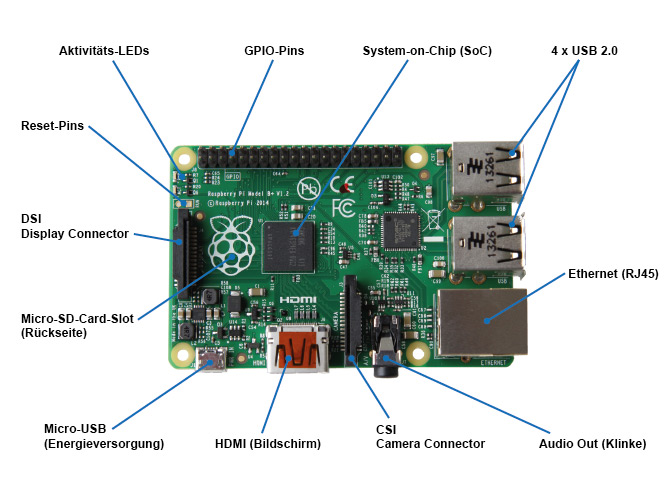
\includegraphics[scale=0.5]{raspberry_pi_3b}
	    				\caption{Raspberry Pi 3b - Quelle: \cite{Picture_Raspberrypi3b} }
	    				\label{raspberrypi3b}
				\end{figure}
				Technische Spezifikationen unseres Raspberry Pi 3b:
				\begin{itemize}
					\item Quad Core 1.2GHz Broadcom BCM2837 64bit CPU
					\item 1GB RAM
					\item BCM43438 wireless LAN and Bluetooth Low Energy (BLE) on board
					\item 100 Base Ethernet
					\item 40-pin extended GPIO
					\item 4 USB 2 ports
					\item 4 Pole stereo output and composite video port
					\item Full size HDMI
					\item CSI camera port for connecting a Raspberry Pi camera
					\item DSI display port for connecting a Raspberry Pi touchscreen display
					\item Micro SD port for loading your operating system and storing data
					\item Upgraded switched Micro USB power source up to 2.5A
				\end{itemize}
			\subsection{Raspberry Pi Shield - Display LCD-Touch, 3,2in}
				Der Touchscreen wertet den Raspberry Pi zu einem vollwertigen Touch-PC auf. Für zusätzliche Funktionen besitzt der Display 3 Buttons an der Seite, welche einfach über die GPIO Pins eingelesen werden können.
				\begin{figure}[ht]
					\centering
					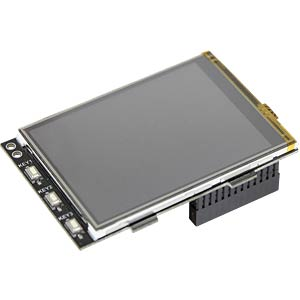
\includegraphics[scale=0.5]{touch_display}
					\caption{Touchscreen Display für den Raspberry Pi - Quelle: \cite{Picture_touchdisplay}}
					\label{touchdisplay}
				\end{figure}
				Technische Spezifikationen unseres Raspberry Pi Shield - Display LCD-Touch, 3.2in:
				\begin{itemize}
					\item Display 8,13cm (3,2")
					\item Auflösung 320 x 240 Pixel
					\item LED-Hintergrundbeleuchtung
					\item 3 frei belegbare Taster (angebunden an GPIO12, 16, 18)
					\item SPI-Schnittstelle
					\item Touchscreen Technologie resistiv
				\end{itemize}
			\subsection{SD-Karte}
    			Die SD-Karte ist eine SanDisk extreme mit einer Speicherkapazität von 32GB. Sie dient als Speichermedium des Raspberry Pi's. Zu Beginn wird das Betriebssystem auf die Karte geflasht von dieser wird der Einplatinencomputer gebooted.

    			
    	\section{Software}
    		\subsection{balenaEtcher}
    			Flash Sd Card
    		\subsection{hostapd}
        		Mit hostapd ist es möglich Geräte, die ein WLAN-Modul besitzen als Access Point zu betreiben. Jedoch können keine Einstellungen im Bereich IP und Routing vorgenommen werden. Die Software ist nur für das Erstellen eines "wireless Ethernet switches" zuständing. \cite{Quote_hostapd1} 
    		\subsection{dnsmasq}
        		Geräte in einem Netzwerk benötigen zur Kommunikation eine IP Adresse und einen DNS Server für die Namensauflösung. Deshalb muss in diesem Projekt ein DHCP und DNS erstellt werden. Von diesen bekommen die Endgeräte ihre IP Konfiguration im WLAN. Die Software dnsmasq wird in diesem Projekt verwerdet um dies zu ermöglichen.
    		\subsubsection{netfilter-persistent und iptables-persistent}
        		Für die Druchführung des Projektes ist es nötig iptable-Regeln anzulegen. Diese sollten nach einem Neustart nicht neu angelegt werden müssen. Deshalb wurden die Pakete netfilter-persistent und iptables-persistent installliert. Damit können die Regeln in eine Datei abgespeichert und beim Neustart automatisch geladen werden.
    		\subsection{cron}
			Planen der Ausführung des Skripts
    		\subsection{Python3.7}
    			Für die Skripte zur Passwortgenerierung, QR-Code Generierung und zum Einlesen der Buttons wird die Sprache Python verwendet. Python 3.7 kommt ist bei Raspbian vorinstalliert und erleichtert durch verschiedene Bibliotheken die Umsetzung des Projektes.
    			\subsubsection{pyqrcode}
    			\subsubsection{gpiozero}
    	
    	
    	\section{Vorbereitung des Raspberry Pi}
    	\subsection{Auswahl und Installation des Betriebssystem}
    	Um mit dem Projekt beginnen zu können musste zuerst ein Betriebssystem bestimmt werden.
    	Es wurde sich für das Raspberry Pi OS Lite entschieden. Begründet wurde diese Entscheidung  durch die weniger vorinstallierten Pakete und einer fehlender grafischen Bedienoberfälche. Hierdurch konnte Speicherplatz und Sicherheitsrisiken eingespart werden. Je weniger unbenützte Software, desto weniger Angriffsfläche. \\ \\
    	
    	Nach der Auswahl des Betriebsystems konnte dieses auf eine SD-Karte geschrieben werden.
    	Hierzu wurde die Software balenaEtcher verwendet.   
    	
    	
    	\subsection{Aktualisierung und Paketinstallation}
    	Nach der Neuinstallation eines Betriebsystems fehlt diesem oft die aktuellsten Versionen von Softwarpaketen und Updates. Deshalb wurde diese zuerst aktuallisiert und installiert. So werden Konflikte aufgrund veraltete Software vermieden und die Sicherheit verbessert.  
    	Darauf folgte das Nachinstallieren der für das Projekt noch benötigten Pakete. Diese wurden im Abschnitt Software genauer beschrieben. 
    	
    	
    	\subsection{SSH Zugriff einrichten}
    	Da das Projektteam aus drei Personen besteht, wurde ein SSH Zugriff in den Einstellungen des Raspberry Pi eingerichtet. Die Einstellungen könne mit folgendem Befehl geöffnet werden: 
    	\lstset{
        language=bash,
        keywordstyle=\color{blue},
        commentstyle=\color{dkgreen},
        numbers=left,
        basicstyle=\scriptsize\ttfamily,
        showspaces=false,
        frame= single,
        xleftmargin=0.5cm
        }

        \begin{lstlisting}
sudo raspi-config
        \end{lstlisting} 
    	
        In diesem Zuge wurde das der SSH Zugriff aktiviert und das Standardpasswort geändert. Durch den SSH Zugriff konnte das parallele Arbeiten am Projekt ermöglicht werden. 
    	
    	\section{Konfiguration des RaspberryPi als funktionalen Access-Point}
            \subsection{WLAN Interface}
            \subsection{Routing}
            \subsection{DNS und DHCP}
            \subsection{Access Point Einstellungen}
         
            
    	\section{Passwortgenerierung}
    		Die Passwortgenerierung wird mithilfe eines Python Skripts gelöst. Dieses ist in unserem GitHub repository hinterlegt und für jeden zugänglich (ref zum Link). Das Skript verwendet die zwei Imports string und secrets. Mithilfe der Bibliothek string können die für Bash problematischen Zeichen aus dem Alphabet entfernt werden. Das secrets Modul wird für das Generieren von stark kryptographischen Passwörter verwendet. Die verwendete Funktion secrets.choice wählt aus der mitgelieferten Sequenz ein zufälliges Zeichen aus. Welches anschließend an den schon vorhandenen String angehängt wird. Dies wird 10 mal wiederholt.
    	
    	\lstset{
    			numbers=left,
    			basicstyle=\ttfamily,
    			language=Python,
    			keywordstyle=\color{blue},
    			commentstyle=\color{green},
    			xleftmargin=1cm
    		}
    	
    	
    	
\begin{lstlisting}
import secrets
import string

def get_random_password():
temp = string.ascii_letters + string.digits 
+ string.punctuation

alphabet = temp.replace('\'', '')
.replace('\\', '')
.replace('\"','').replace('\`', '')
.replace(';', '')

password = ''.join(secrets
.choice(alphabet) for i in range(10))
return password

if __name__ == "__main__":
print(get_random_password())
\end{lstlisting}
    	
    	\section{Ausgabe des Passworts}
    	
    	
    	
    	\section{Fazit mit Ausblick}
    	
    	\section{Quellenverzeichnis}
        \bibliography{zitate}
        \bibliographystyle{plain}
    	
\end{document}
